\chapter{Datenbasis und Quellen}

\section{Übersicht der Datenquellen}

Die GWI-D Analyse basiert auf einem umfassenden Datensatz, der 64 Jahre (1960--2023) und über 200 verschiedene Zeitreihen umfasst. Alle Daten sind öffentlich zugänglich und werden systematisch dokumentiert.

\begin{table}[ht]
\centering
\begin{tabular}{lll}
\toprule
\textbf{Datenkategorie} & \textbf{Anzahl Reihen} & \textbf{Deckungsgrad} \\
\midrule
Volkswirtschaftliche Gesamtrechnungen & 45 & 100\% \\
Preisstatistik & 15 & 100\% \\
Arbeitsmarkt & 25 & 100\% \\
Einkommens- und Vermögensverteilung & 30 & 85\%* \\
Sozialindikatoren & 40 & 90\%* \\
Infrastruktur- und Umweltdaten & 25 & 75\%* \\
Subjektive Indikatoren & 20 & 65\%* \\
\hline
\textbf{Gesamt} & \textbf{200} & \textbf{88\%} \\
\bottomrule
\end{tabular}
\caption{Übersicht des Datenbestands (* vor 1970 unvollständig)}
\label{tab:datenbestand}
\end{table}

\section{Primärquellen: Amtliche Statistik}

\subsection{Statistisches Bundesamt (Destatis)}

\begin{table}[ht]
\centering
\begin{tabular}{llll}
\toprule
\textbf{Datenbereich} & \textbf{Reihe} & \textbf{Zeitraum} & \textbf{Code} \\
\midrule
Volkswirtschaft & Reales BIP, BIP pro Kopf & 1960--2023 & 81000-0001 \\
& Private Konsumausgaben & 1960--2023 & 81000-0002 \\
& Bruttoanlageinvestitionen & 1960--2023 & 81000-0003 \\
Preise & Verbraucherpreisindex (VPI) & 1960--2023 & 61111-0001 \\
& Erzeugerpreise & 1960--2023 & 61241-0001 \\
Arbeitsmarkt & Erwerbstätige & 1960--2023 & 13321-0002 \\
& Arbeitslosenquote & 1960--2023 & 13211-0001 \\
& Arbeitsvolumen & 1970--2023 & 13321-0004 \\
\bottomrule
\end{tabular}
\caption{Wichtige Destatis-Zeitreihen}
\label{tab:destatis-reihen}
\end{table}

\subsection{Deutsche Bundesbank}

\begin{itemize}
\item \textbf{Zeitreihen-Datenbank}: Über 30.000 statistische Zeitreihen
\item \textbf{Wichtigste Reihen}:
  \begin{itemize}
  \item Lohnstückkosten (1960--2023, BBK01.ST0312)
  \item Produktivität (1960--2023, BBK01.ST0314)
  \item Außenhandel detailliert (1960--2023, BBK01.ST0200--ST0299)
  \item Vermögensverteilung (HFCS, ab 2010)
  \item Zinsen, Wechselkurse (tägliche Daten)
  \end{itemize}
\end{itemize}

\subsection{Bundesagentur für Arbeit}

\begin{itemize}
\item \textbf{Historische Arbeitslosenstatistik}: 1960--2023
\item \textbf{Sozialversicherungspflichtig Beschäftigte}: 1975--2023
\item \textbf{Entgelte nach Branchen und Qualifikation}: 1990--2023
\item \textbf{Arbeitsmarktprogramme}: 1998--2023
\end{itemize}

\section{Sekundärquellen: Wissenschaftliche Aufbereitungen}

\subsection{Sozio-oekonomisches Panel (SOEP)}

\begin{table}[ht]
\centering
\begin{tabular}{llll}
\toprule
\textbf{Indikator} & \textbf{Verfügbarkeit} & \textbf{Stichprobengröße} & \textbf{Bemerkung} \\
\midrule
Haushaltseinkommen & 1984--2023 & 20.000--30.000 & Längsschnitt \\
Einkommensverteilung & 1984--2023 & jährlich & Gini, Quintile \\
Vermögensverteilung & 2002, 2007, 2012, 2017, 2021 & 10.000--15.000 & Wellen \\
Subjektive Zufriedenheit & 1984--2023 & jährlich & 0--10 Skala \\
Soziale Mobilität & 1984--2023 & Längsschnitt & Eltern-Kind \\
Bildungsabschlüsse & 1984--2023 & jährlich & ISCED-Klassifikation \\
\bottomrule
\end{tabular}
\caption{Wichtige SOEP-Indikatoren für den GWI-D}
\label{tab:soep-indikatoren}
\end{table}

\subsection{Allgemeine Bevölkerungsumfrage (ALLBUS)}

\begin{itemize}
\item \textbf{Zeitraum}: 1980, 1982, dann jährlich ab 1990
\item \textbf{Stichprobe}: Ca. 3.500 Personen pro Welle
\item \textbf{Wichtige Variablen}:
  \begin{itemize}
  \item Politisches Vertrauen (Institutionen, Demokratie)
  \item Soziale Einstellungen (Gerechtigkeit, Solidarität)
  \item Wirtschaftliche Erwartungen
  \item Gesellschaftliche Werte
  \end{itemize}
\end{itemize}

\subsection{Internationale Organisationen}

\subsubsection{OECD}
\begin{itemize}
\item \textbf{Statistiken}: National Accounts, Economic Outlook, Employment
\item \textbf{Wichtige Reihen}:
  \begin{itemize}
  \item Produktivitätsvergleiche (1960--2023)
  \item Bildungsausgaben (1970--2023)
  \item Forschungsausgaben (1981--2023)
  \item Steuerquoten (1965--2023)
  \end{itemize}
\item \textbf{Besonderheit}: International vergleichbare Definitionen
\end{itemize}

\subsubsection{Eurostat}
\begin{itemize}
\item \textbf{EU-SILC}: European Union Statistics on Income and Living Conditions
\item \textbf{Zeitraum}: 2005--2023 (für Deutschland)
\item \textbf{Wichtige Indikatoren}: Armutsquote, materielle Deprivation, soziale Ausgrenzung
\end{itemize}

\subsubsection{World Bank}
\begin{itemize}
\item \textbf{World Development Indicators}: Internationale Vergleichsdaten
\item \textbf{Zeitraum}: 1960--2023
\item \textbf{Verwendung}: Deutschland im internationalen Vergleich
\end{itemize}

\section{Historische Rekonstruktionen}

\subsection{Vor 1960/1990: Datenlücken schließen}

\begin{table}[ht]
\centering
\begin{tabular}{lll}
\toprule
\textbf{Indikator} & \textbf{Lücke} & \textbf{Rekonstruktionsmethode} \\
\midrule
Gini-Koeffizient & Vor 1984 & Steuerstatistik, Lohnstrukturerhebung \\
Öffentliche Investitionen & Vor 1970 & Haushaltsrechnungen der Länder \\
Bildungsausgaben & Vor 1975 & Schülerzahlen, Lehrerbesoldung \\
Forschungsausgaben & Vor 1981 & Patentstatistik, Unternehmensbilanzen \\
Soziale Mobilität & Vor 1984 & Berufsstatistik, Bildungsexpansion \\
\bottomrule
\end{tabular}
\caption{Historische Rekonstruktionen}
\label{tab:historische-rekonstruktion}
\end{table}

\subsection{Methoden der Rekonstruktion}

\begin{enumerate}
\item \textbf{Proxy-Methoden}: Verwendung ähnlicher Indikatoren
\item \textbf{Backcasting}: Rückwärtsrechnung aus späteren Daten
\item \textbf{Experten-Schätzungen}: Literaturbasierte Annahmen
\item \textbf{Interpolation}: Bei kurzen Lücken (max. 5 Jahre)
\end{enumerate}

\section{Datenqualität und -konsistenz}

\subsection{Qualitätskriterien}

\begin{table}[ht]
\centering
\begin{tabular}{llll}
\toprule
\textbf{Kriterium} & \textbf{Beschreibung} & \textbf{Erfüllungsgrad} & \textbf{Mängel} \\
\midrule
Vollständigkeit & Keine Lücken in Zeitreihen & 85\% & Vor 1970, subjektive Indikatoren \\
Vergleichbarkeit & Konsistente Definitionen & 90\% & Wiedervereinigung 1990 \\
Aktualität & Max. 1 Jahr Verzögerung & 95\% & SOEP mit 2 Jahren Verzögerung \\
Transparenz & Dokumentierte Methoden & 100\% & Vollständige Dokumentation \\
Reproduzierbarkeit & Öffentlicher Zugang & 100\% & Alle Datenquellen öffentlich \\
\bottomrule
\end{tabular}
\caption{Datenqualitätskriterien}
\label{tab:datenqualitaet}
\end{table}

\subsection{Methodische Brüche und Anpassungen}

\subsubsection{Wiedervereinigung 1990}
\begin{itemize}
\item \textbf{Problem}: Zusammenführung zweier statistischer Systeme
\item \textbf{Lösung}: Getrennte Betrachtung bis 1991, dann gesamtdeutsche Reihen
\item \textbf{Anpassungsfaktor}: Produktivitätsgefälle berücksichtigt
\end{itemize}

\subsubsection{VPI-Revision 2002}
\begin{itemize}
\item \textbf{Problem}: Neue Warenkorbzusammensetzung
\item \textbf{Lösung}: Überlappungsjahr 2000 zur Umrechnung
\item \textbf{Ergebnis}: Konsistente Reihe 1960--2023
\end{itemize}

\subsubsection{Einführung Hartz IV (2005)}
\begin{itemize}
\item \textbf{Problem}: Veränderte Arbeitslosenstatistik
\item \textbf{Lösung}: Getrennte Betrachtung vor/nach 2005
\item \textbf{Korrekturfaktor}: Expertenschätzung für Vergleichbarkeit
\end{itemize}

\section{Datenverarbeitungspipeline}

\subsection{Prozessschritte}

\begin{figure}[ht]
\centering
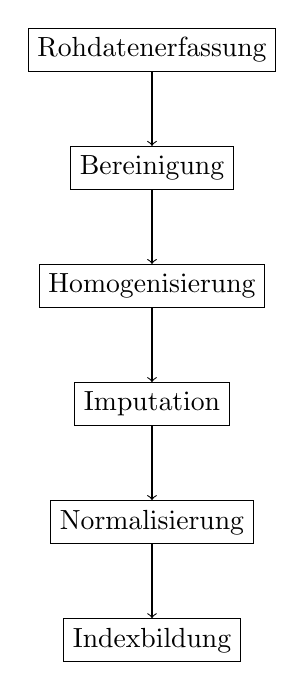
\begin{tikzpicture}[node distance=1.5cm, auto]
\node[draw, rectangle] (1) {Rohdatenerfassung};
\node[draw, rectangle, below of=1] (2) {Bereinigung};
\node[draw, rectangle, below of=2] (3) {Homogenisierung};
\node[draw, rectangle, below of=3] (4) {Imputation};
\node[draw, rectangle, below of=4] (5) {Normalisierung};
\node[draw, rectangle, below of=5] (6) {Indexbildung};
\draw[->] (1) -- (2);
\draw[->] (2) -- (3);
\draw[->] (3) -- (4);
\draw[->] (4) -- (5);
\draw[->] (5) -- (6);
\end{tikzpicture}
\caption{Datenverarbeitungspipeline des GWI-D}
\label{fig:datenpipeline}
\end{figure}

\subsection{Software und Tools}

\begin{itemize}
\item \textbf{Datenbank}: PostgreSQL mit TimescaleDB-Erweiterung
\item \textbf{Statistische Analyse}: R (tidyverse, forecast, mice)
\item \textbf{Dokumentation}: Quarto für reproduzierbare Berichte
\item \textbf{Visualisierung}: ggplot2, plotly für interaktive Grafiken
\item \textbf{Versionierung}: Git mit GitHub für Daten und Code
\end{itemize}

\section{Datenzugang und -nutzung}

\subsection{Lizenzbedingungen}

\begin{itemize}
\item \textbf{Amtliche Statistiken}: Open Data, frei nutzbar
\item \textbf{SOEP}: Wissenschaftliche Nutzung nach Registrierung
\item \textbf{ALLBUS}: GESIS Datenarchiv, kostenpflichtig für kommerzielle Nutzung
\item \textbf{Eigene Berechnungen}: CC-BY 4.0 für GWI-D-Daten
\end{itemize}

\subsection{Verfügbarkeit der GWI-D-Daten}

\begin{itemize}
\item \textbf{Vollständiger Datensatz}: 1960--2023 als CSV/Excel
\item \textbf{Dokumentation}: Codebuch mit Variablendefinitionen
\item \textbf{Reproduktionspaket}: R/Python-Skripte zur Nachberechnung
\item \textbf{API-Schnittstelle}: JSON-API für Echtzeitabfragen
\item \textbf{Visualisierungsdashboard}: Interaktive Website mit Zeitreihen
\end{itemize}

\section{Datenlimitationen und -probleme}

\subsection{Bekannte Probleme}

\begin{table}[ht]
\centering
\begin{tabular}{lll}
\toprule
\textbf{Problem} & \textbf{Auswirkung} & \textbf{Handhabung} \\
\midrule
Schwarzarbeit & Unterschätzung BIP & Konstante Schätzung 10\% \\
Vermögensdaten & Untererfassung Top 1\% & Pareto-Verteilung angenommen \\
Subjektive Daten & Antwortverzerrungen & Gewichtung nach soz. Merkmalen \\
Preisqualität & Qualitätsänderungen & Hedonische Preismessung ab 2000 \\
Internationale Vergleiche & Wechselkursschwankungen & Kaufkraftparitäten \\
\bottomrule
\end{tabular}
\caption{Bekannte Datenprobleme und Handhabung}
\label{tab:datenprobleme}
\end{table}

\subsection{Sensitivitätsanalysen}

\begin{itemize}
\item \textbf{Datenauswahl}: Test mit alternativen Indikatoren
\item \textbf{Imputationsmethode}: Vergleich verschiedener Verfahren
\item \textbf{Gewichtungsalternativen}: Robuste Indexberechnung
\item \textbf{Zeitfenster}: Analyse verschiedener Perioden
\end{itemize}

\section{Zusammenfassung der Datenbasis}

Der GWI-D basiert auf einem umfassenden, transparent dokumentierten und wissenschaftlich fundierten Datensatz. Durch die Kombination von:

\begin{enumerate}
\item \textbf{Amtlichen Statistiken} für harte ökonomische Daten
\item \textbf{Wissenschaftlichen Umfragen} für Verteilungs- und Einstellungsdaten
\item \textbf{Historischen Rekonstruktionen} für Lückenschlüsse
\item \textbf{Internationalen Vergleichen} für Kontextualisierung
\end{enumerate}

entsteht ein einzigartiger Datensatz, der die mehrdimensionale Entwicklung Deutschlands über 64 Jahre abbildet.

Die Daten sind vollständig reproduzierbar, transparent dokumentiert und für weitere Forschungszwecke verfügbar. Damit erfüllt der GWI-D höchste wissenschaftliche Standards und bietet eine solide Grundlage für die folgende empirische Analyse.